\documentclass[compress]{beamer}
\usepackage{ifthen,verbatim}

\title{Effect of Muon Alignment on TeV tracks}
\author{Jim Pivarski, Alexei Safonov}
\institute{Texas A\&M University}
\date{29 October, 2007}

\newcommand{\isnote}{}
\xdefinecolor{lightyellow}{rgb}{1.,1.,0.25}
\xdefinecolor{darkblue}{rgb}{0.1,0.1,0.7}

%% Uncomment this to get annotations
%% \def\notes{\addtocounter{page}{-1}
%%            \renewcommand{\isnote}{*}
%% 	   \beamertemplateshadingbackground{lightyellow}{white}
%%            \begin{frame}
%%            \frametitle{Notes for the previous page (page \insertpagenumber)}
%%            \itemize}
%% \def\endnotes{\enditemize
%% 	      \end{frame}
%%               \beamertemplateshadingbackground{white}{white}
%%               \renewcommand{\isnote}{}}

%% Uncomment this to not get annotations
\def\notes{\comment}
\def\endnotes{\endcomment}

\setbeamertemplate{navigation symbols}{}
\setbeamertemplate{headline}{\includegraphics[height=1 cm]{../cmslogo} \hspace{0.1 cm} \includegraphics[height=1 cm]{../tamulogo} \hfill
\begin{minipage}{5.5 cm}
\vspace{-0.75 cm} \small
\begin{center}
\ifthenelse{\equal{\insertpagenumber}{1}}{}{\textcolor{blue}{\insertsection}}
\end{center}
\end{minipage} \hfill
\begin{minipage}{4.5 cm}
\vspace{-0.75 cm} \small
\begin{flushright}
\ifthenelse{\equal{\insertpagenumber}{1}}{}{Jim Pivarski \hspace{0.5 cm} \insertpagenumber\isnote/\pageref{numpages}}
\end{flushright}
\end{minipage}\mbox{\hspace{0.2 cm}}}

\begin{document}
\frame{\titlepage}

\begin{frame}
\hspace{-0.83 cm} \textcolor{darkblue}{\Large Context}

\vspace{0.1 cm}
\begin{itemize}\setlength{\itemsep}{0.1 cm}
\item We have been developing a muon alignment procedure in the
CSC DPG and the Alignment \& Calibration groups
\item Baseline procedure has stabilized, ready to be applied to physics
\end{itemize}

\vfill
\hspace{-0.83 cm} \textcolor{darkblue}{\Large Outline for this talk}

\vspace{0.1 cm}
\begin{itemize}\setlength{\itemsep}{0.1 cm}
\item Overview of the procedure
\item New set of scenarios, comparable to Muon10InversePb and Muon100InversePb
\item Consequences for physics
\end{itemize}

\label{numpages}
\end{frame}

\section*{Overview of the procedure}

\begin{frame}
\frametitle{Baseline procedure}
%% Developed a basic alignment procedure in the CSC Detector Performance Group
%%     Based on HIP algorithm, using tracker as a reference: converges in 1 iteration
%%     Applies equally to CSC and DT
%%     Uses 5 pb-1 of high-momentum muons from Z, W decays
%%     With an otherwise ideal detector, reaches 100-micron precision in x
%%     Studying systematic effects one by one
%%     Accuracy is still at 100-200 micron level

\vspace{-0.25 cm}
\begin{itemize}\setlength{\itemsep}{0.1 cm}
\item Based on HIP algorithm in the CommonAlignment framework
\item Applies equally to barrel and endcap
\item Breaks circular dependence between track-fitting and alignment by
using tracker as an external reference
\item Reaches 100~$\mu$m accuracy with 5 pb$^{-1}$ of high-momentum muons from $Z$, $W$ decays (apart from systematics)
\item Studying systematic effects one by one
\end{itemize}

\begin{tabular}{p{0.62\linewidth} p{0.35\linewidth}}
Dependence on miscalibration & negligible \\
\ldots on tracker misalignment & $\mathcal{O}(\mbox{200 $\mu$m})$ (next slide) \\
\textcolor{white}{\ldots}on momentum of tracks & radial outliers (backup) \\
\textcolor{white}{\ldots}inclusive sample, backgrounds & \hspace{0.25 cm} {\it to do\ldots} \\
\textcolor{white}{\ldots}mismeasured $\vec{B}(\vec{x})$ & \hspace{0.25 cm} {\it to do\ldots} \\
\textcolor{white}{\ldots}incorrect material budget/distribution & \hspace{0.25 cm} {\it to do\ldots}
\end{tabular}
\end{frame}

\begin{frame}
\vspace{-0.25 cm}
\begin{center}
Dependence on number of muons (local $x$ is global $r\phi$)

\vspace{0.2 cm}
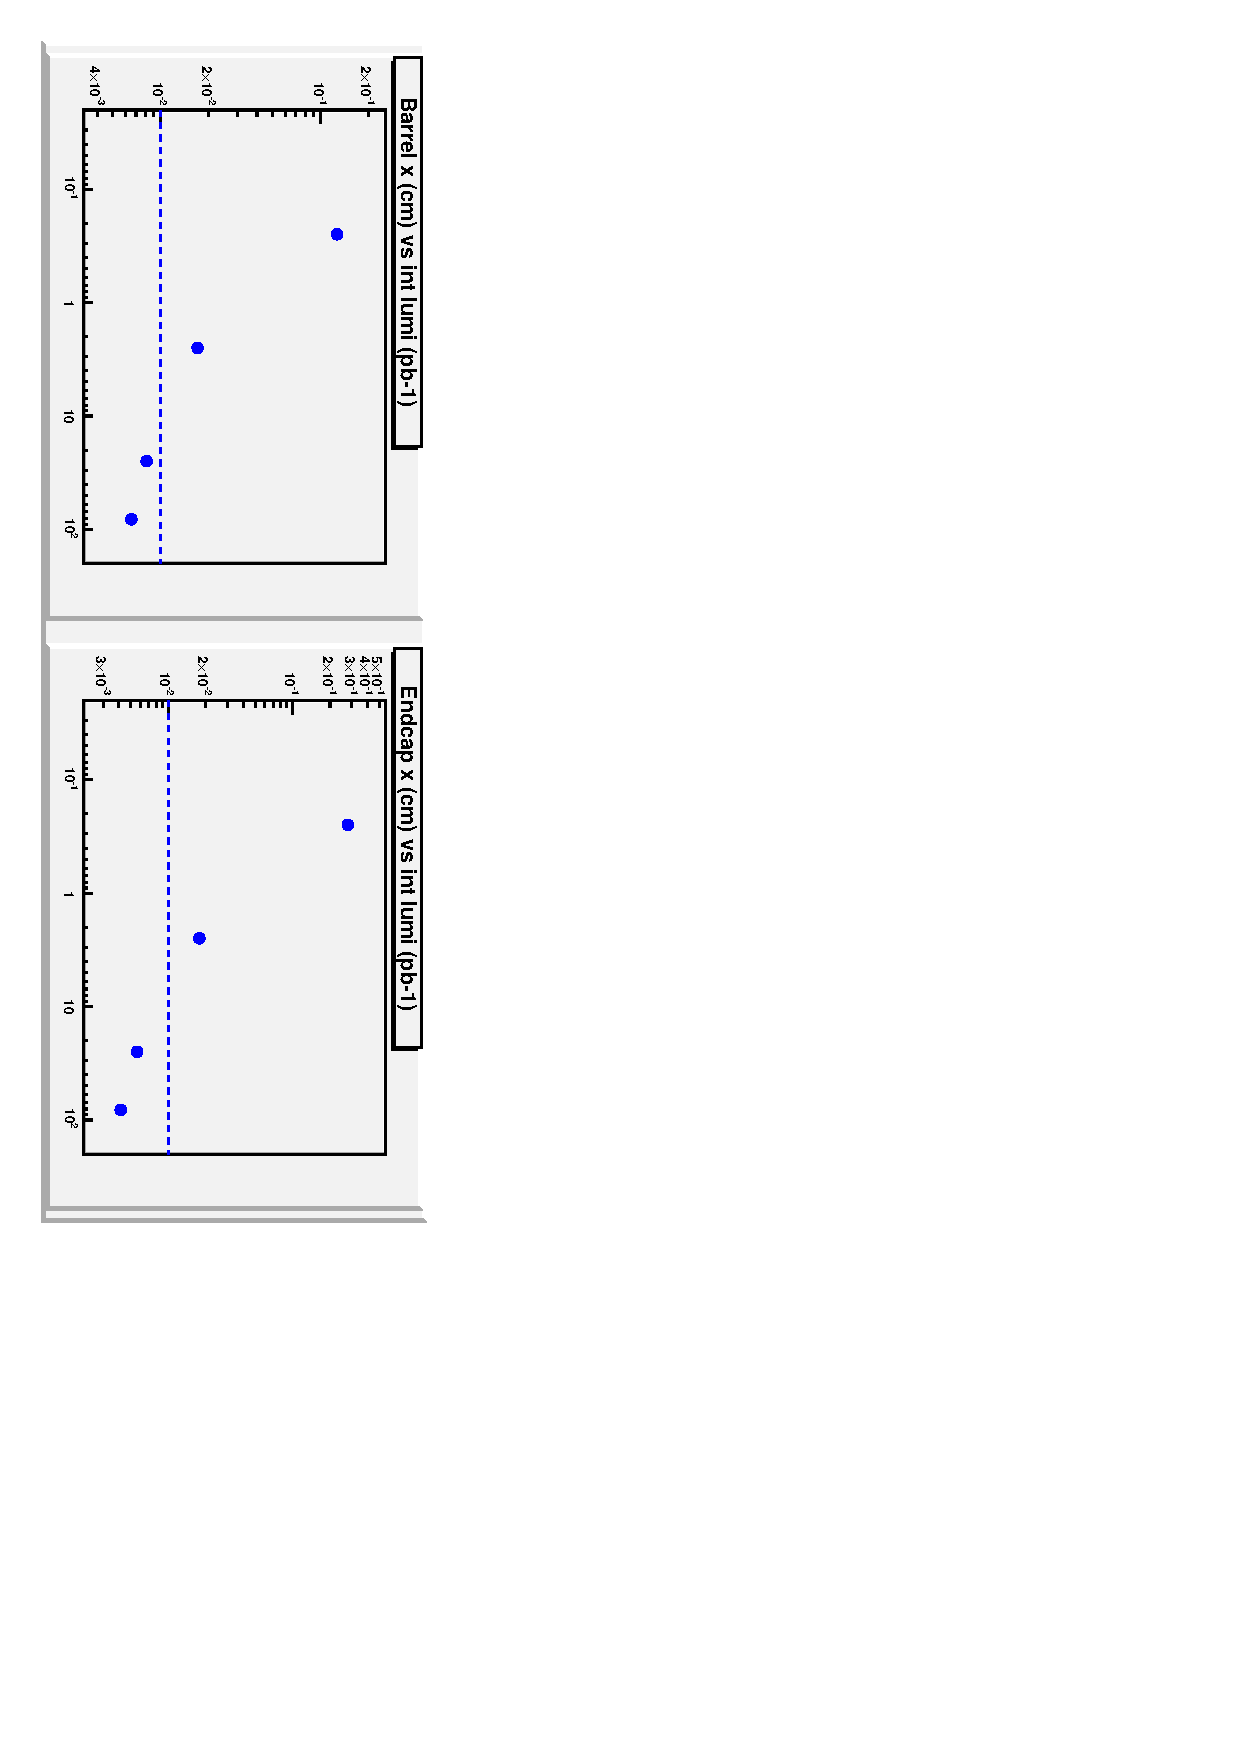
\includegraphics[height=0.9\linewidth, angle=90]{events_x_wacky.pdf}
\end{center}

\begin{center}
Dependence on tracker misalignment (1 = short-term scenario)

\vspace{0.2 cm}
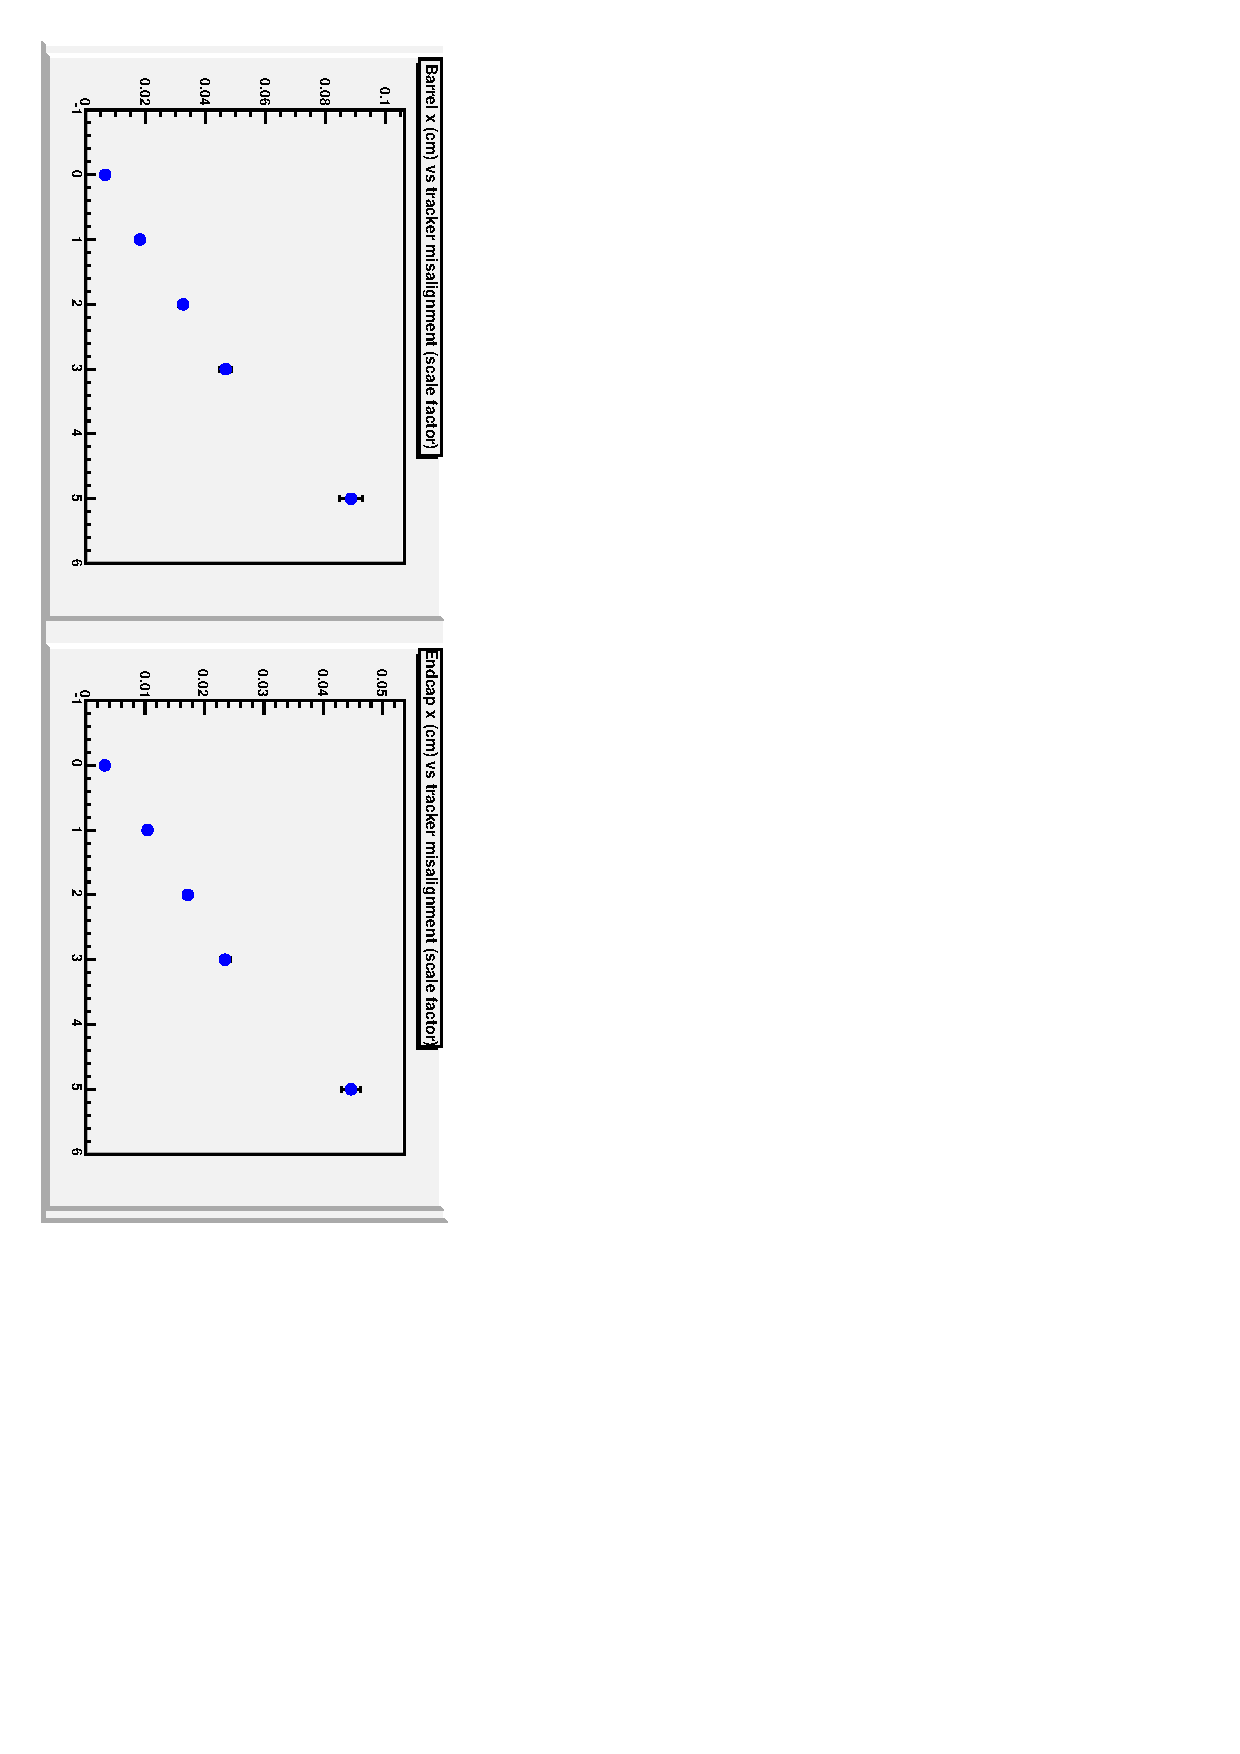
\includegraphics[height=0.9\linewidth, angle=90]{tracker_x_rmsonly.pdf}
\end{center}
\end{frame}

\section*{New set of scenarios}

\begin{frame}
\begin{center}
\Huge \textcolor{blue}{New set of scenarios}
\end{center}

\vspace{1 cm}
\textcolor{darkblue}{\large Alignment simulation output:}
\begin{enumerate}
\item Misalign detector
\item Run alignment procedure under controlled conditions
\item Save output geometry for re-reconstruction
\end{enumerate}
\end{frame}

\begin{frame}
%% Standard 10pb-1, 100pb-1 muon alignment scenarios            Alignment output
%%     conservative estimates                                       realistic output (as realistic as MC)
%%         10pb-1: 2-5 mm wheels/disks, 500 micron chambers             0.8 mm wheels/disks, 100-200 micron chambers
%%         100pb-1: 1 mm wheels/disks, 200 micron chambers
%%     isotropic alignment errors                                   elliptical errors (e.g. x is measured 20 times better than y)
%%     correlations through superstructure hierarchy                correlations from tracks
%%     Gaussian errors                                              not necessarily Gaussian (especially from systematics)

\begin{tabular}{p{0.45\linewidth} p{0.45\linewidth}}
\textcolor{darkblue}{\large Standard scenarios} &
\textcolor{darkblue}{\large Alignment simulation output} \\

\vspace{-0.3 cm}
\begin{itemize}
\item Conservative estimate
\begin{itemize}
\item 2--5 mm wheels/disks, \\ 500~$\mu$m chambers \\ for 10 pb$^{-1}$
\item 1 mm wheels/disks, \\ 200~$\mu$m chambers \\ for 100 pb$^{-1}$
\end{itemize}
\end{itemize} &

\vspace{-0.3 cm}
\begin{itemize}
\item Realistic simulation \\ (as realistic as MC)
\begin{itemize}
\item 0.8 mm wheels/disks, 100--200~$\mu$m chambers

for 5 pb$^{-1}$ of $Z$\&$W$
\end{itemize}
\end{itemize} \\

\vspace{-0.9 cm}
\begin{itemize}
\item isotropic misalignments

\vspace{1 cm}
\item approximate correlations through superstructure hierarchy
\item Gaussian misalignments
\end{itemize} &

\vspace{-0.9 cm}
\begin{itemize}
\item elliptical misalignments (e.g.\ CSC $x$ is measured 20 times better than $y$)
\item correlations from tracks
\item not necessarily Gaussian (especially for systematic effects)
\end{itemize}
\end{tabular}

\vspace{-0.25 cm}
\textcolor{blue}{\scriptsize \tt \href{https://twiki.cern.ch/twiki/bin/view/CMS/SomeSamplesSUSYBSM2007MuonGeometries}{https://twiki.cern.ch/twiki/bin/view/CMS/SomeSamplesSUSYBSM2007MuonGeometries}}
\end{frame}

\section*{Consequences for physics}

\begin{frame}
\begin{center}
\Huge \textcolor{blue}{Consequences for physics}
\end{center}
\end{frame}

%% Applied results of alignment simulation to Z, Z', and Drell-Yan physics samples
%%     visible improvement in Z with standalone, Z' with globalMuon
%%     Z'/DY for systematics studies
%%     momentum resolution as a function of momentum, factorized

%% \begin{frame}
%% \frametitle{Applying alignment results to $Z$, $Z'$, Drell-Yan}
%% \begin{center}
%% Dependence on number of muons

%% \vspace{0.2 cm}
%% \begin{minipage}{\linewidth}
%% \begin{columns}
%% \column{0.5\linewidth}
%% 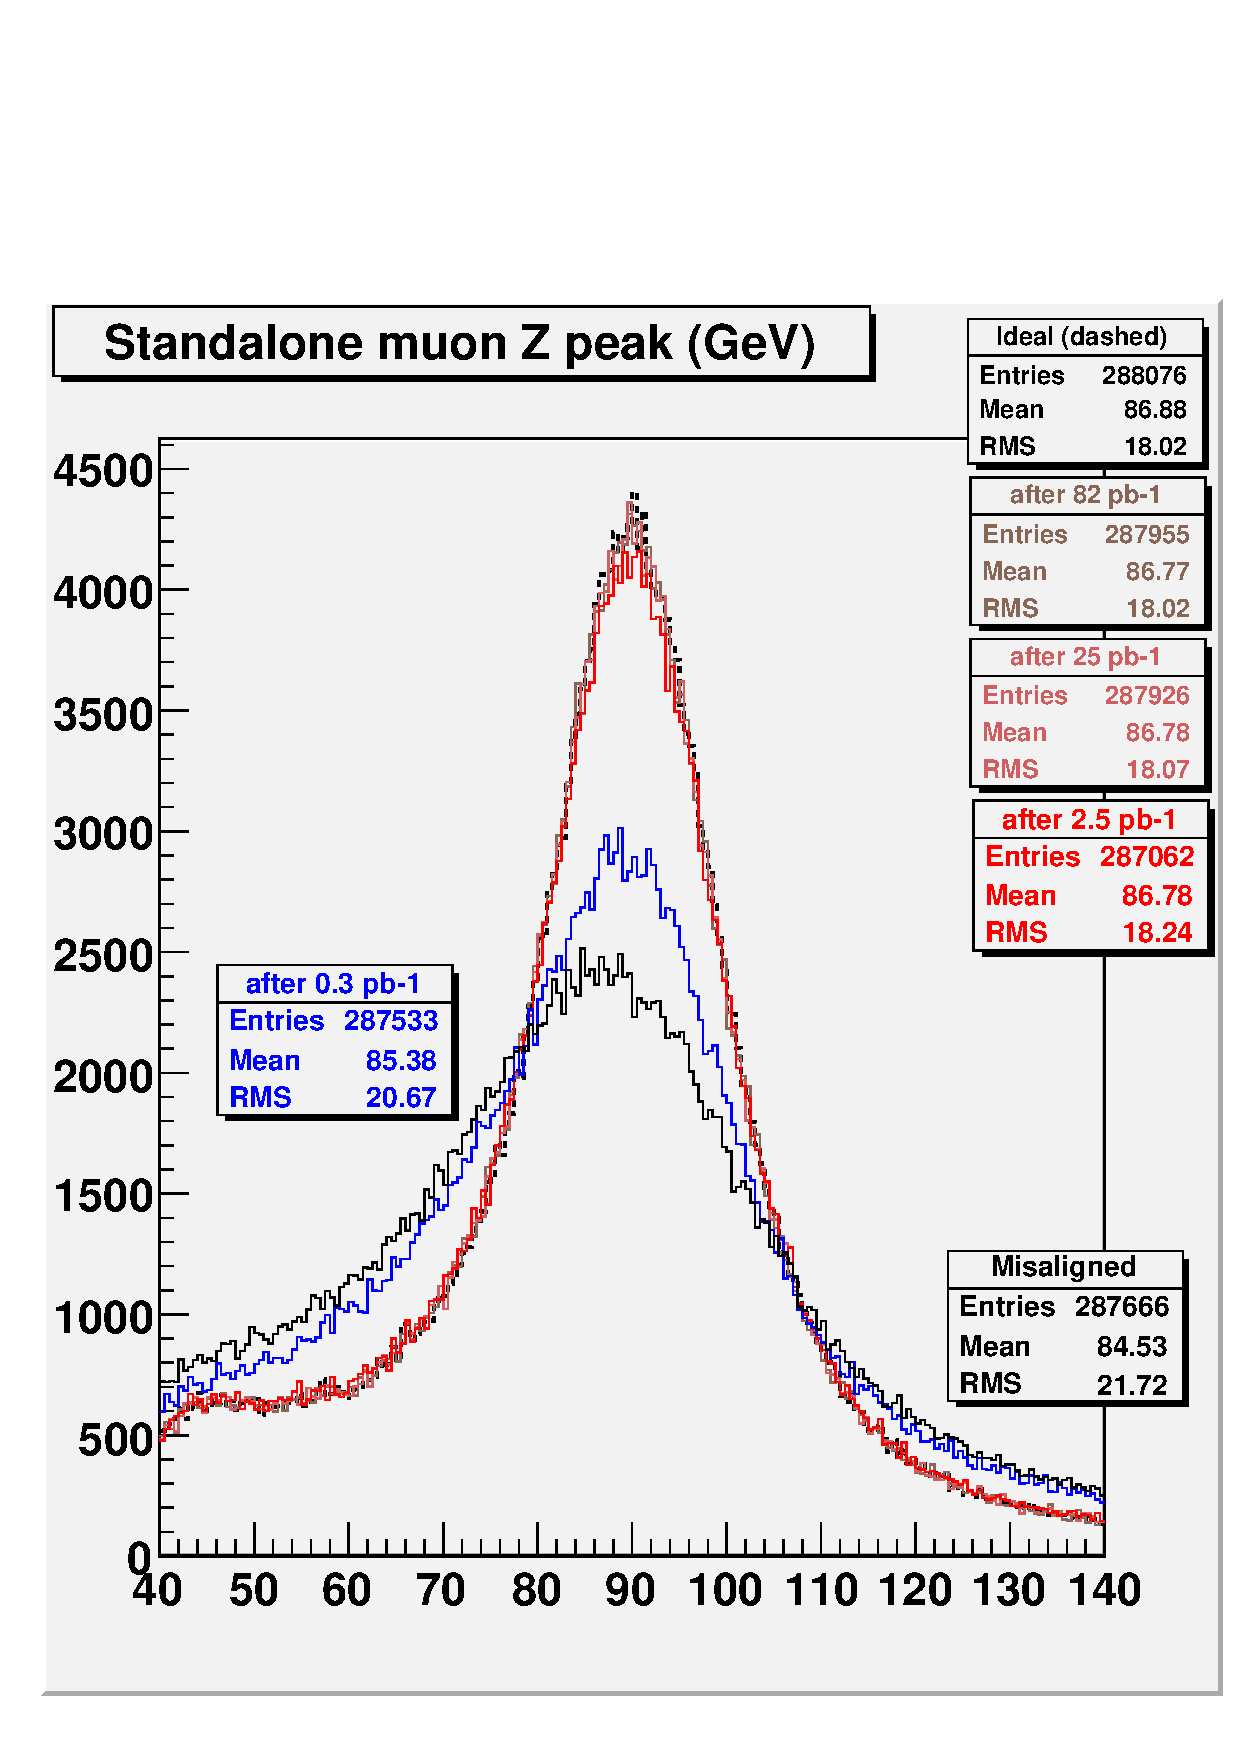
\includegraphics[width=\linewidth]{checkit_standaloneZ.pdf}
%% \column{0.5\linewidth}
%% 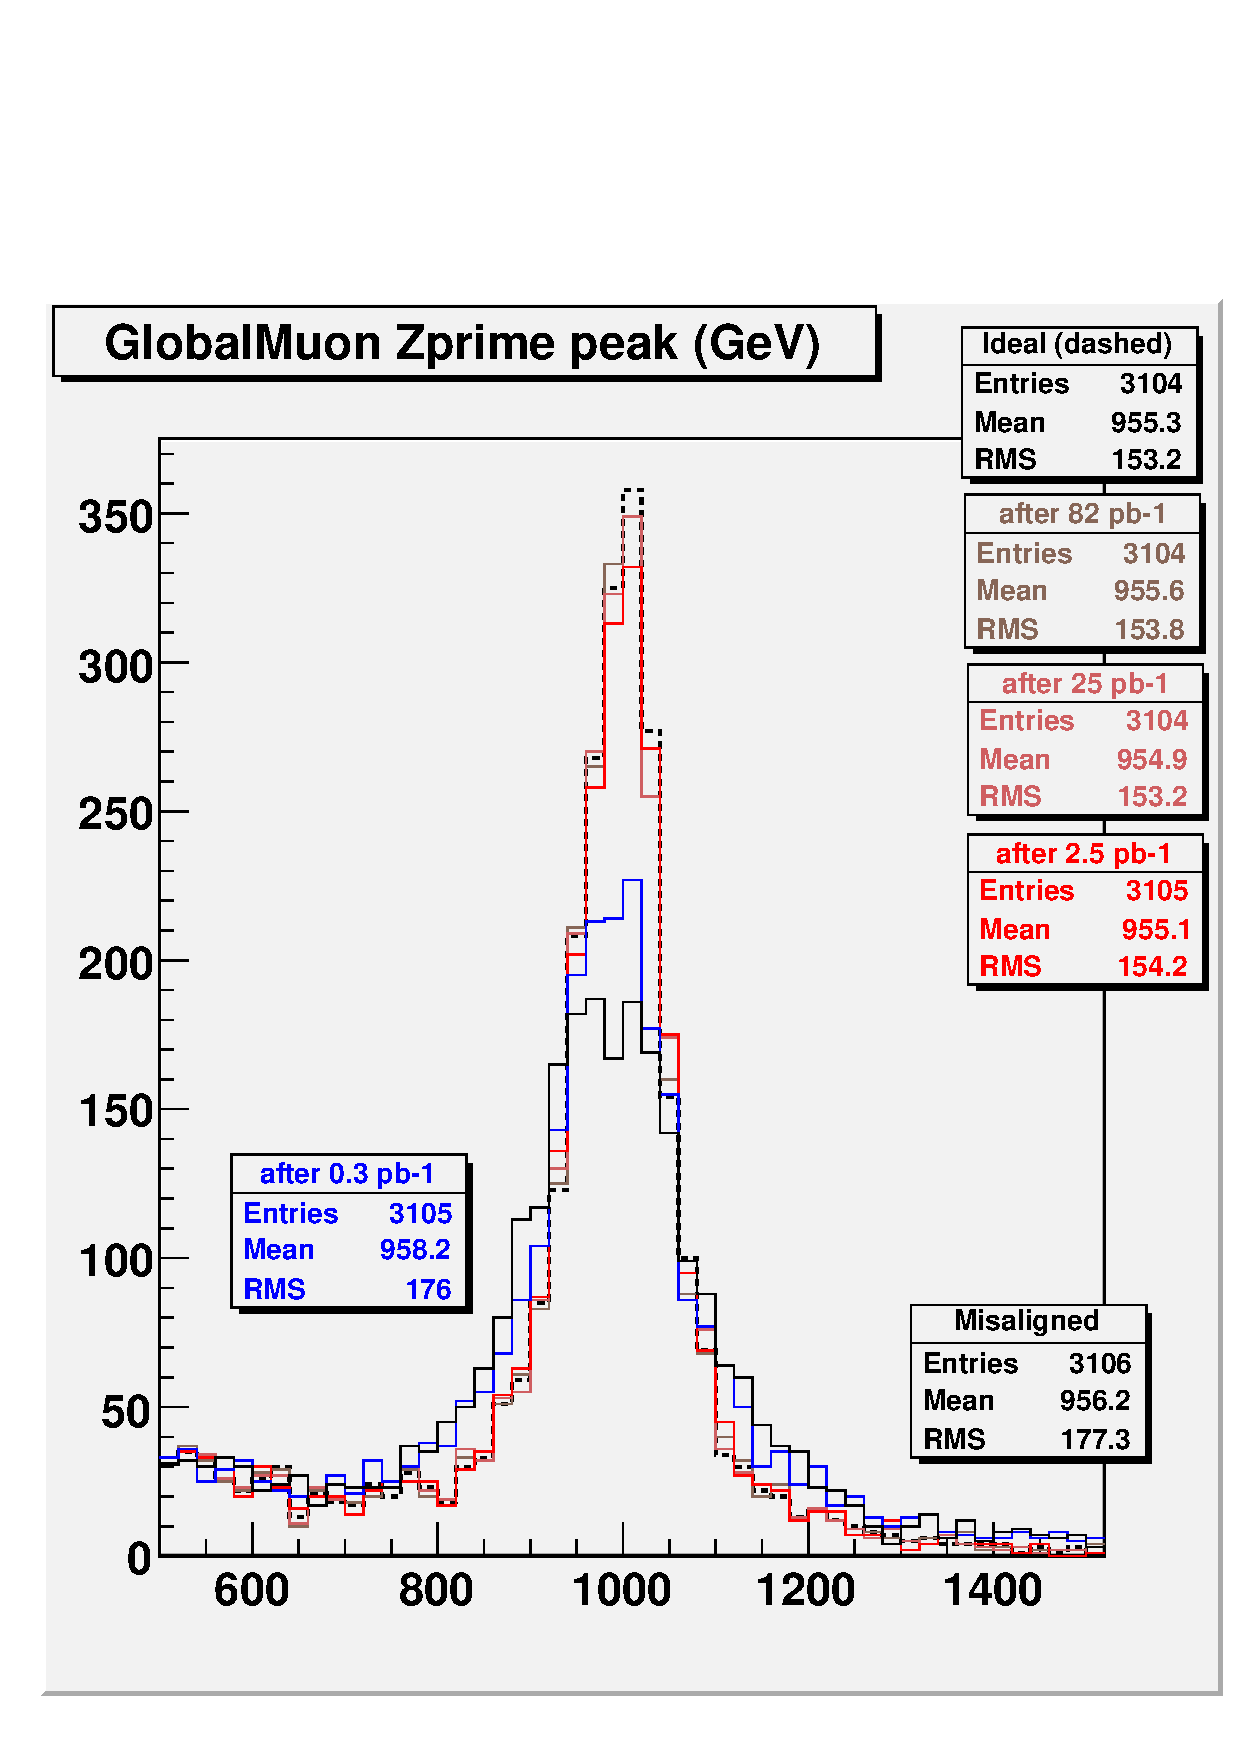
\includegraphics[width=\linewidth]{checkit_globZprime.pdf}
%% \end{columns}
%% \end{minipage}
%% \end{center}
%% \end{frame}

\begin{frame}
\frametitle{Application of new scenarios to \only<2>{2 }TeV Drell-Yan and $Z'$}
\begin{columns}
\column{0.5\linewidth}
\only<1>{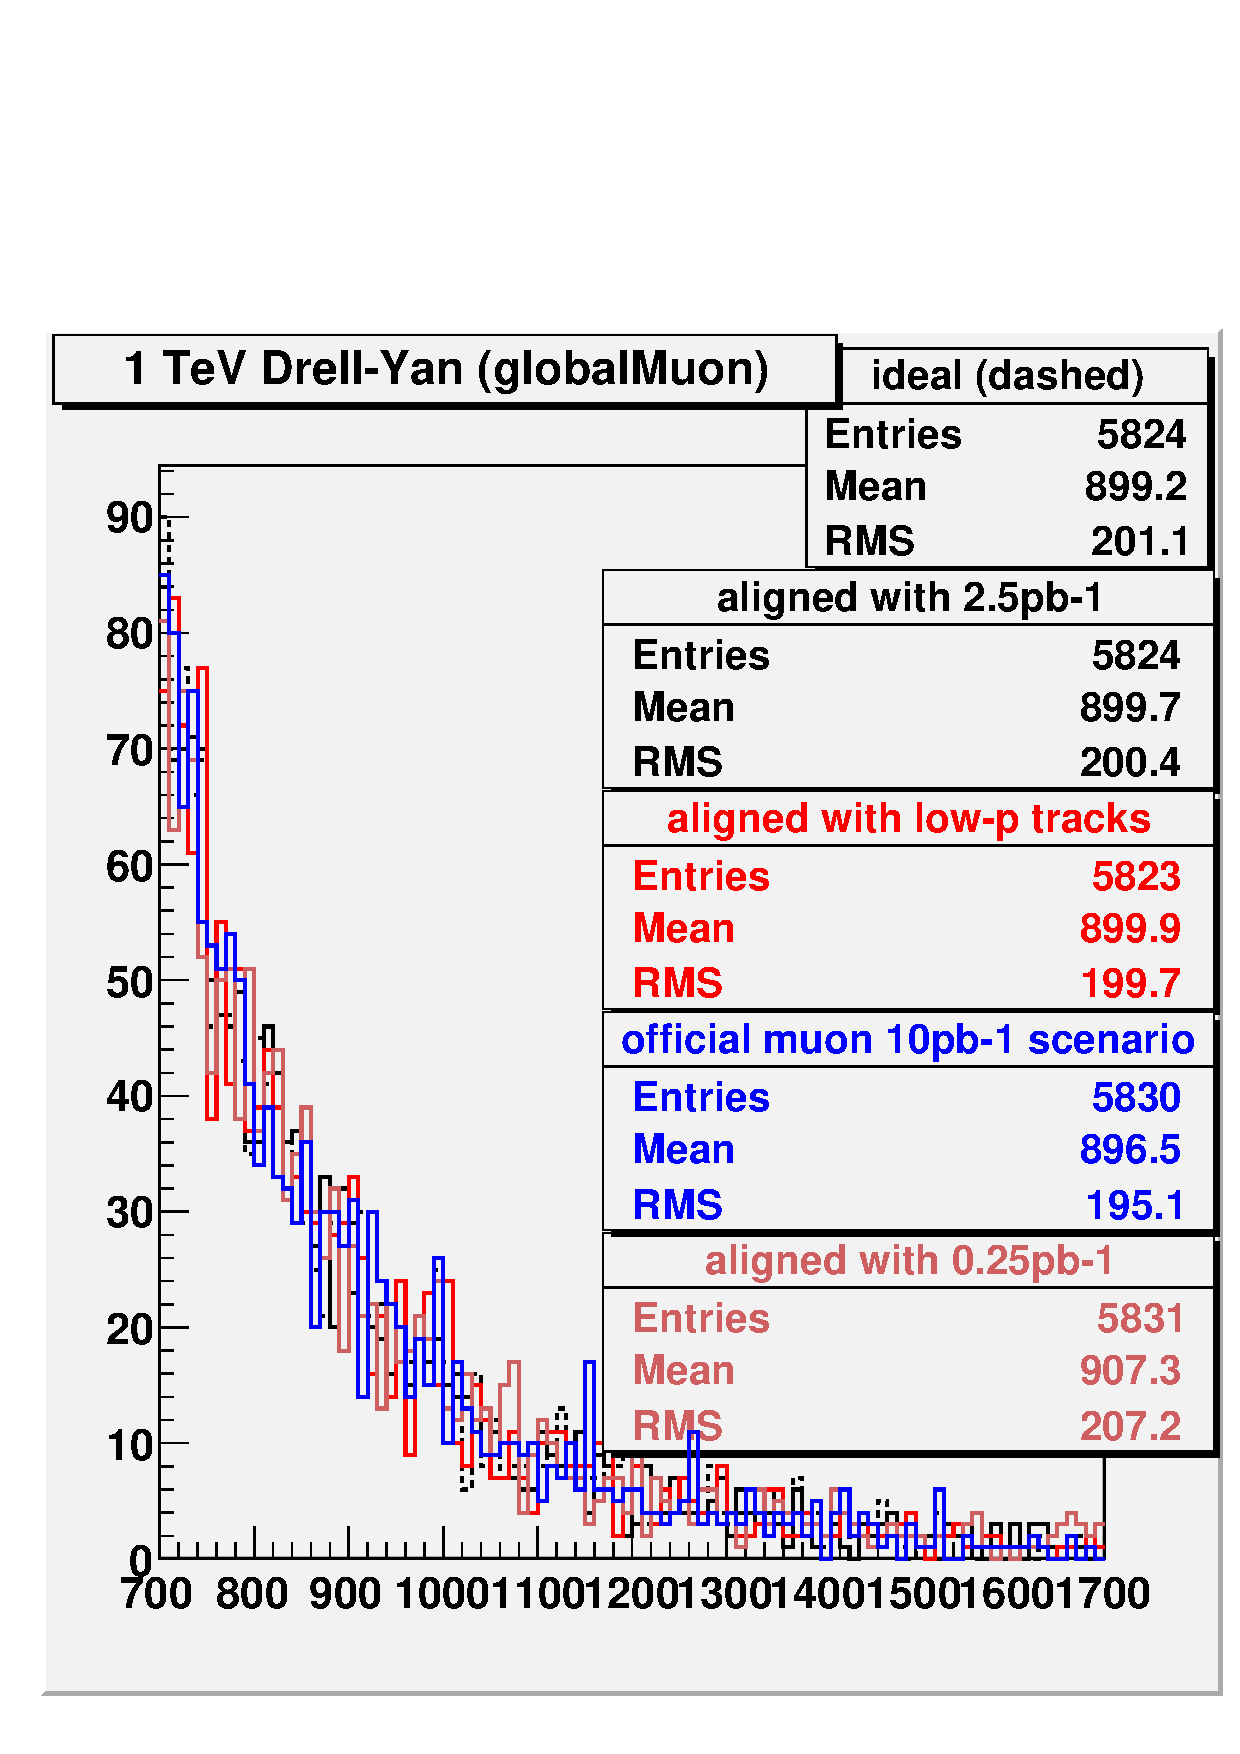
\includegraphics[width=\linewidth]{muoncompare_dy_500.pdf}}
\only<2>{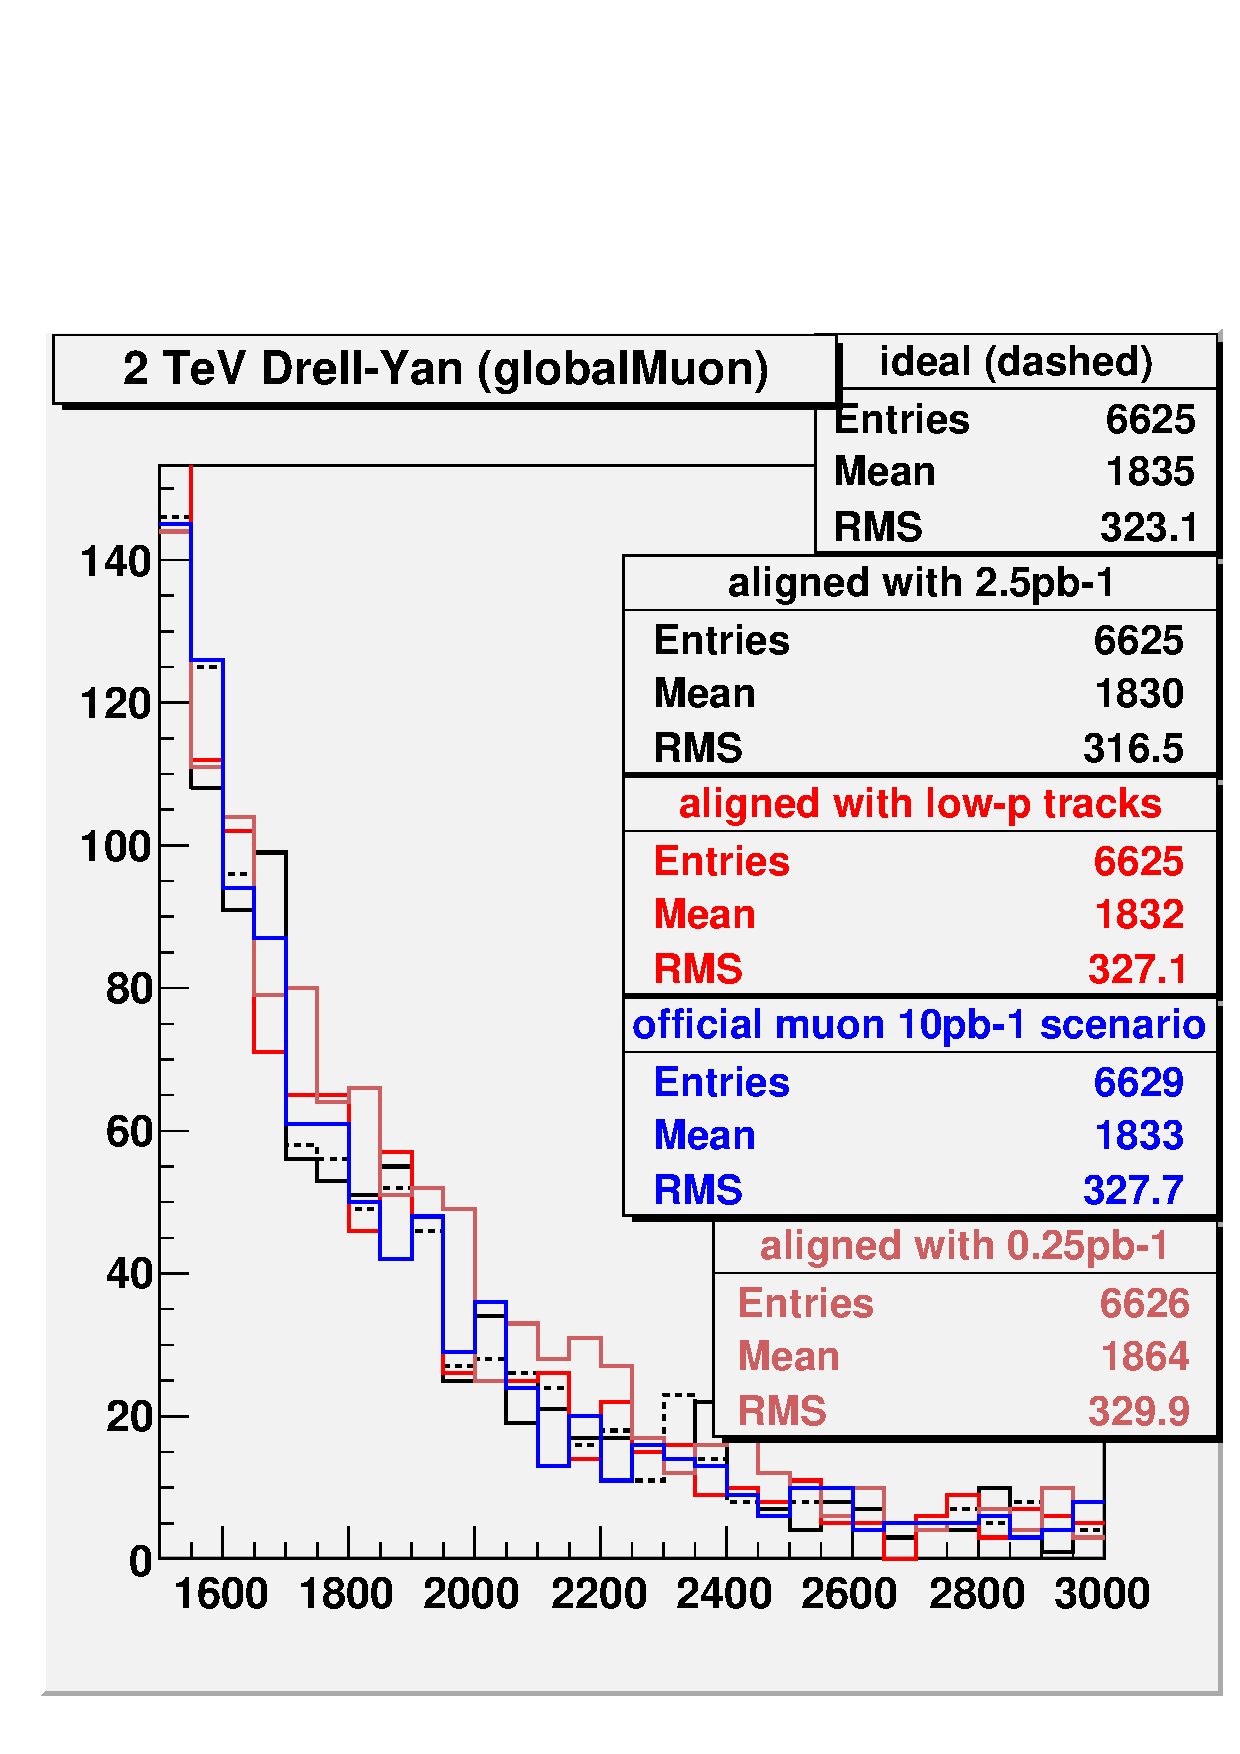
\includegraphics[width=\linewidth]{muoncompare_dy_1000.pdf}}
\column{0.5\linewidth}
\only<1>{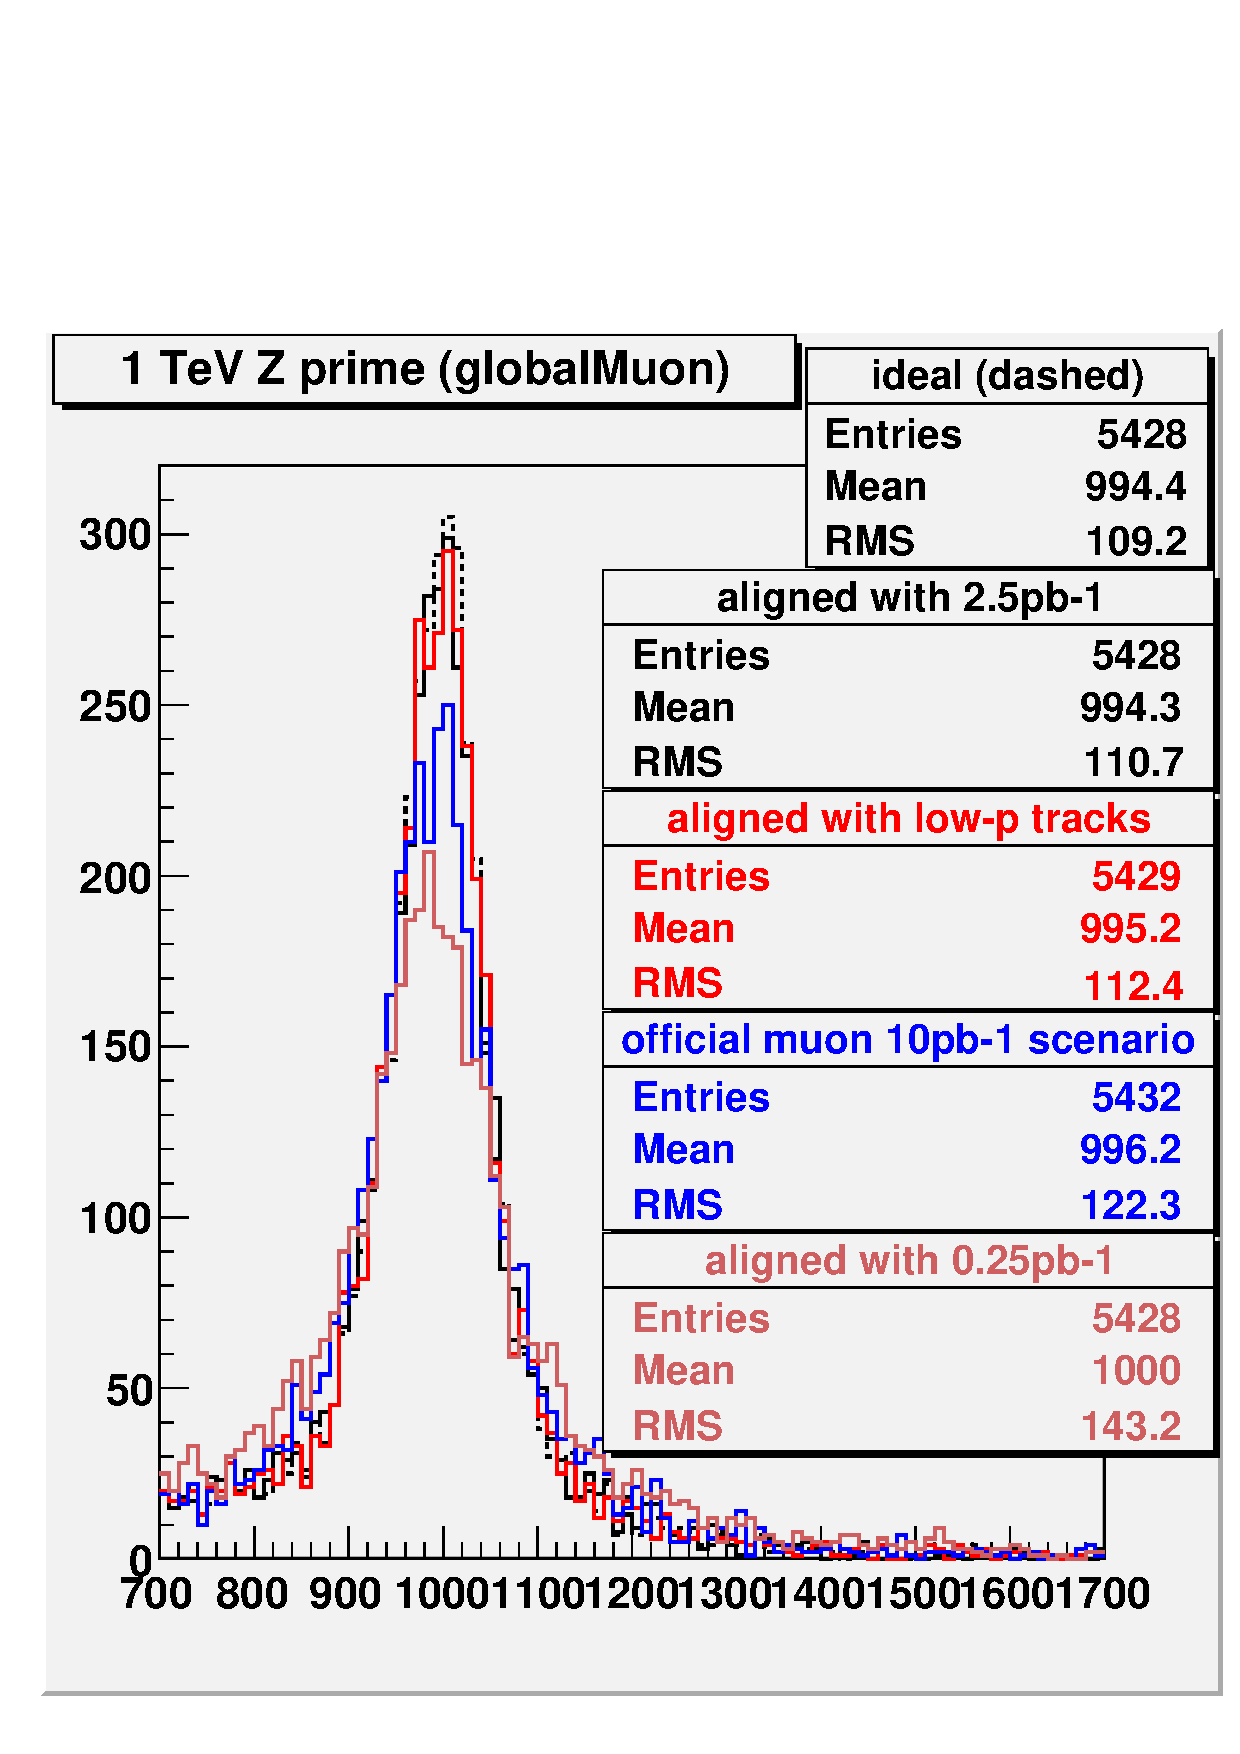
\includegraphics[width=\linewidth]{muoncompare_zprime_1000.pdf}}
\only<2>{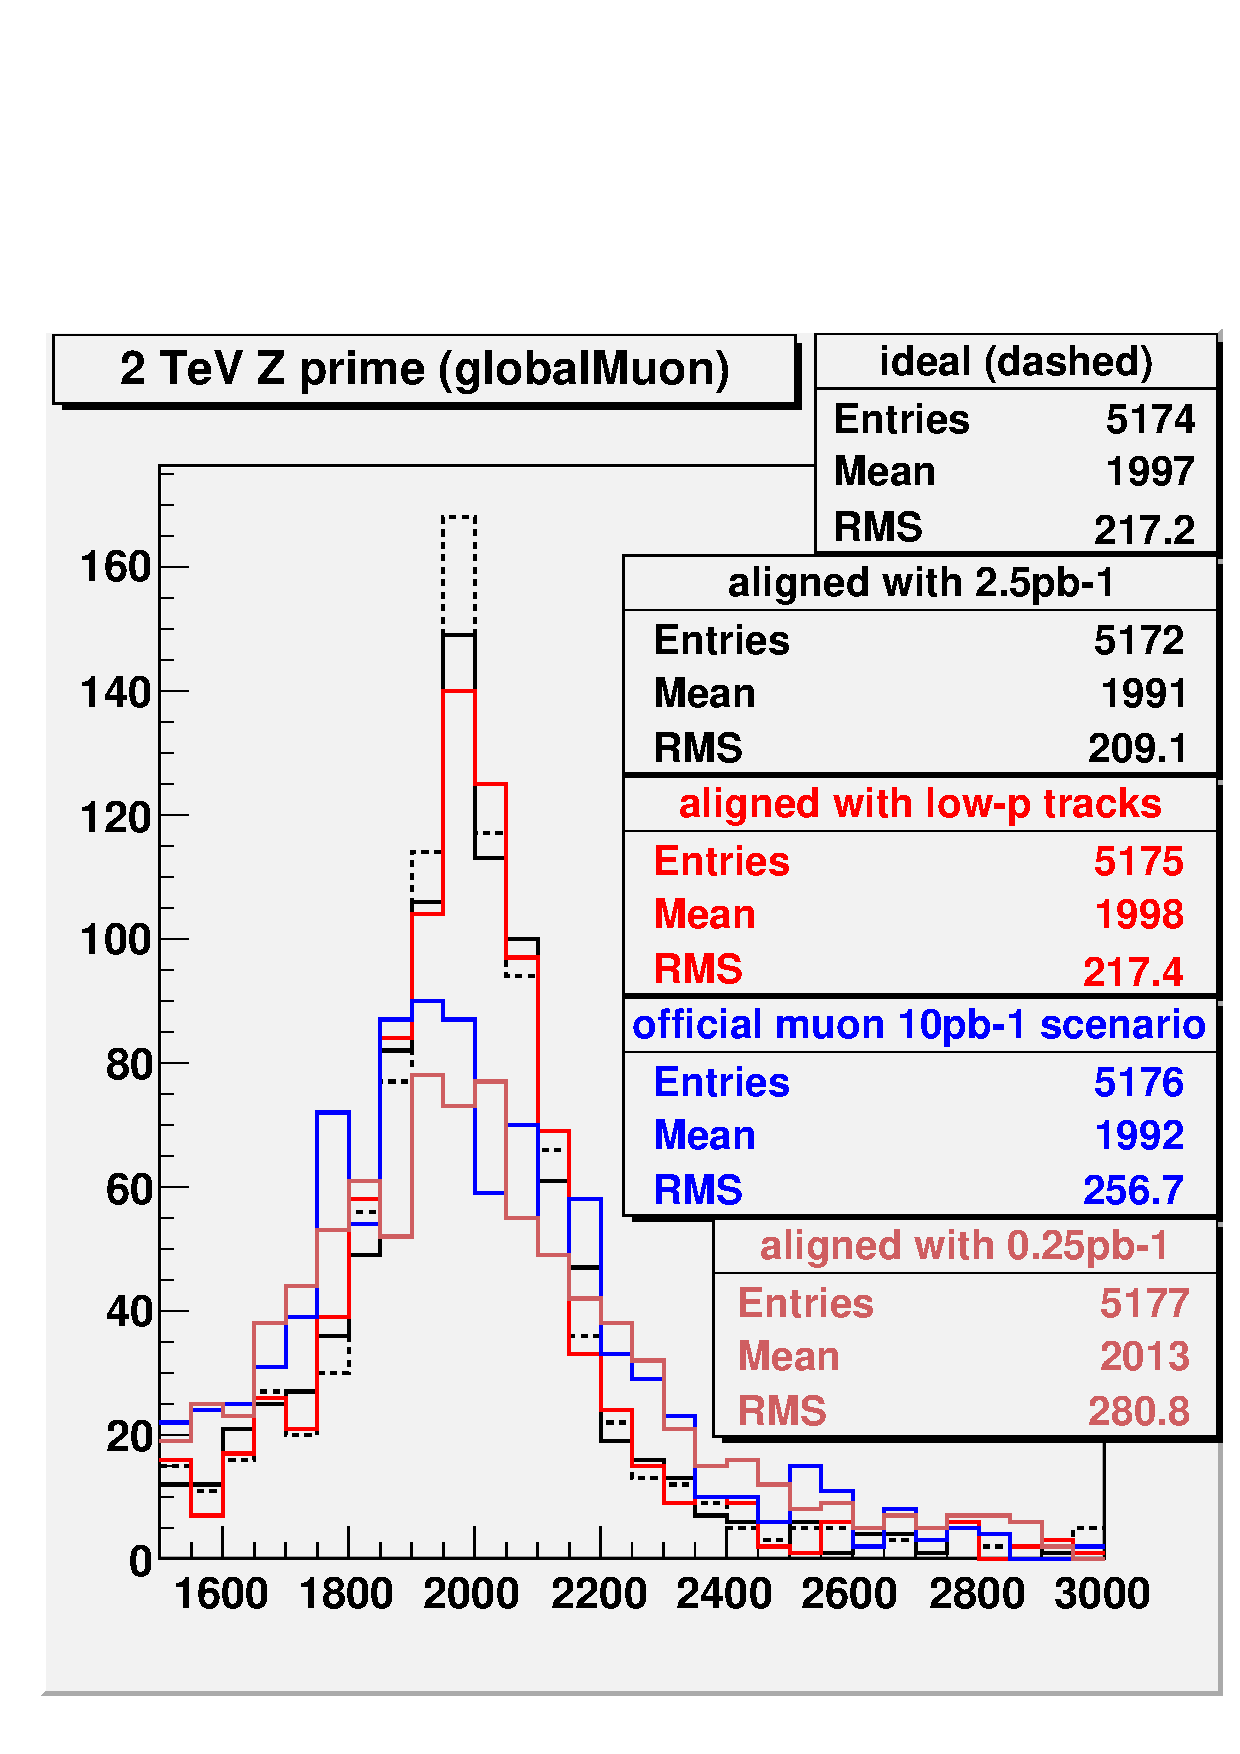
\includegraphics[width=\linewidth]{muoncompare_zprime_2000.pdf}}
\end{columns}

\vspace{0.25 cm}
\textcolor{red}{``low-p'' means 20-60~GeV $Z\to\mu\mu$} \hfill (private 1\_5\_4 $Z'$ samples)

\textcolor{blue}{official 10~pb$^{-1}$ scenario is pessimistic}
\end{frame}

\begin{frame}
\frametitle{Comparison of tracker and muon misalignments (\only<1>{1}\only<2>{2} TeV)}
\begin{columns}
\column{0.5\linewidth}
\hfill \only<1>{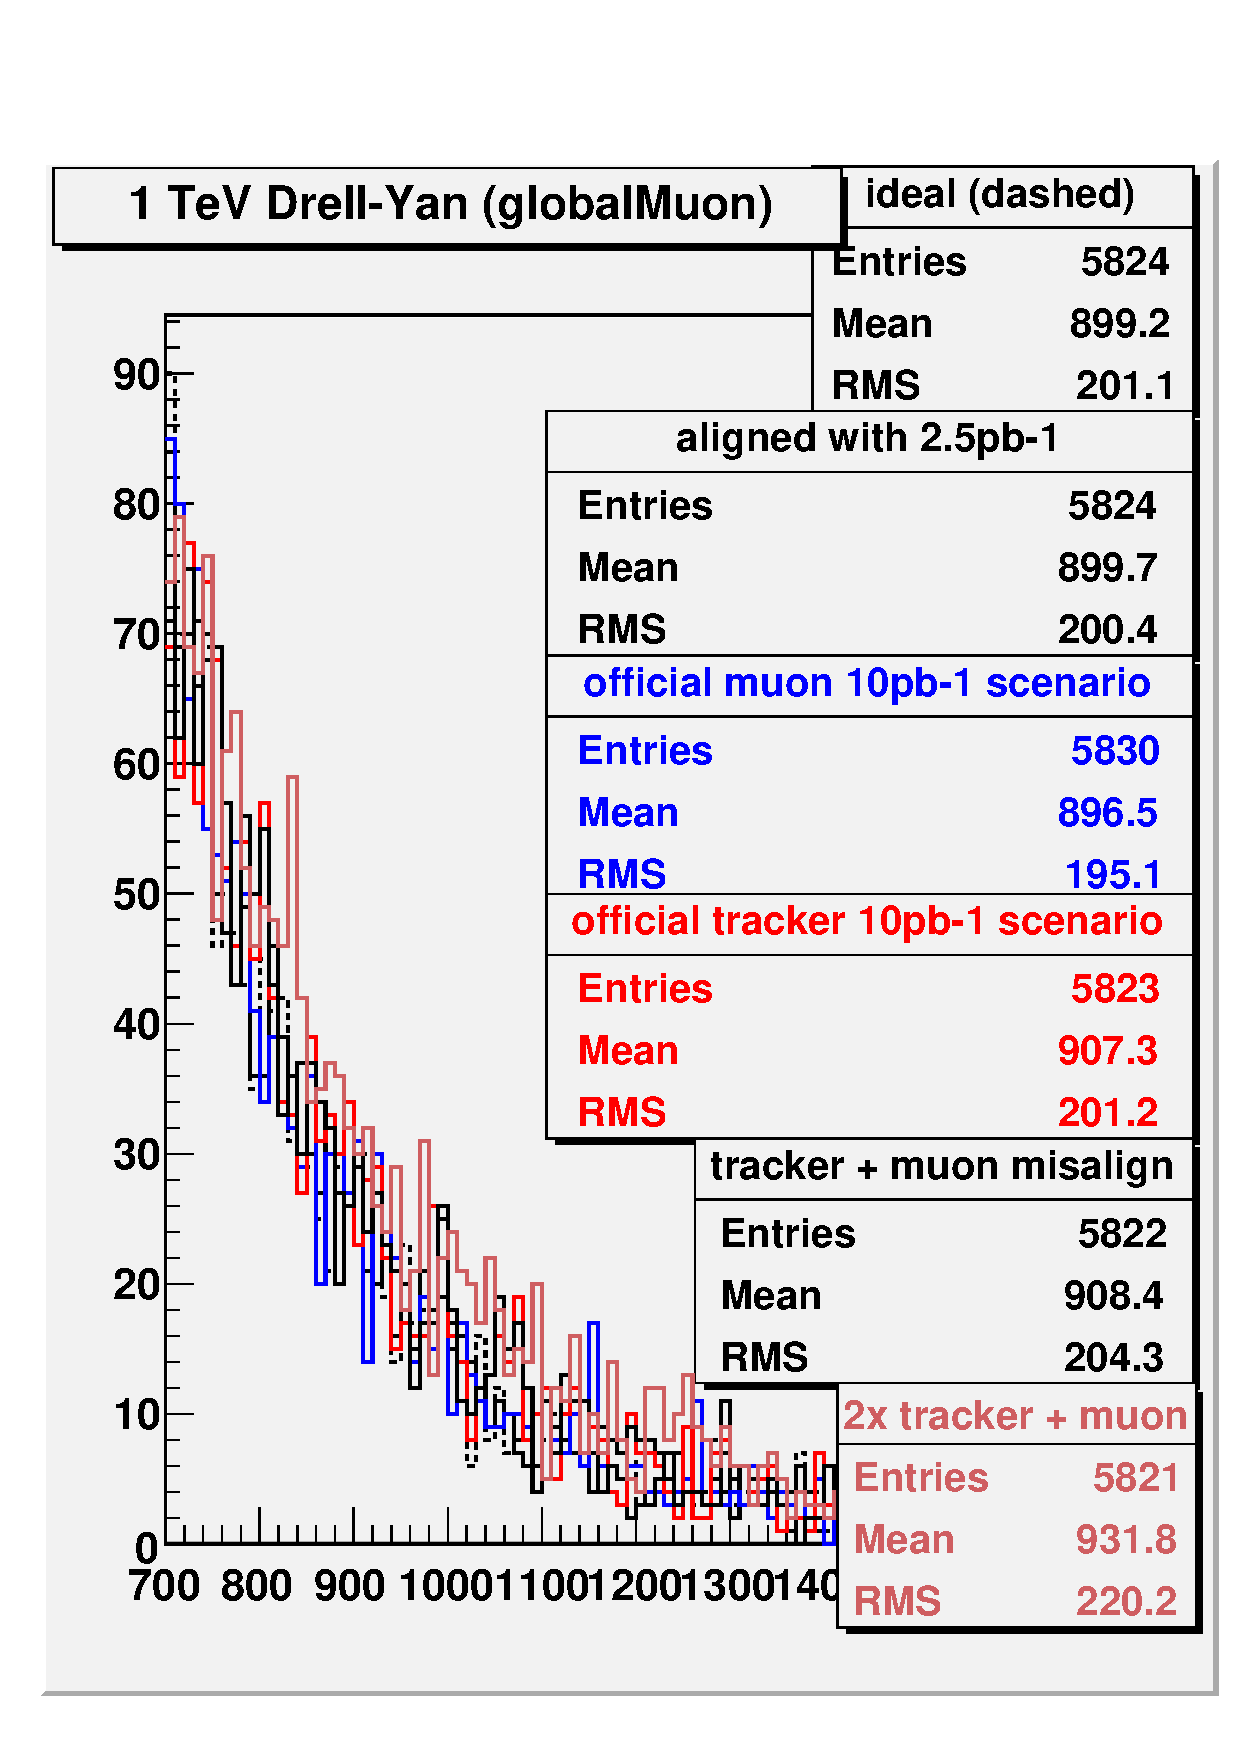
\includegraphics[width=0.85\linewidth]{trackercompare_dy_500.pdf}}
\only<2>{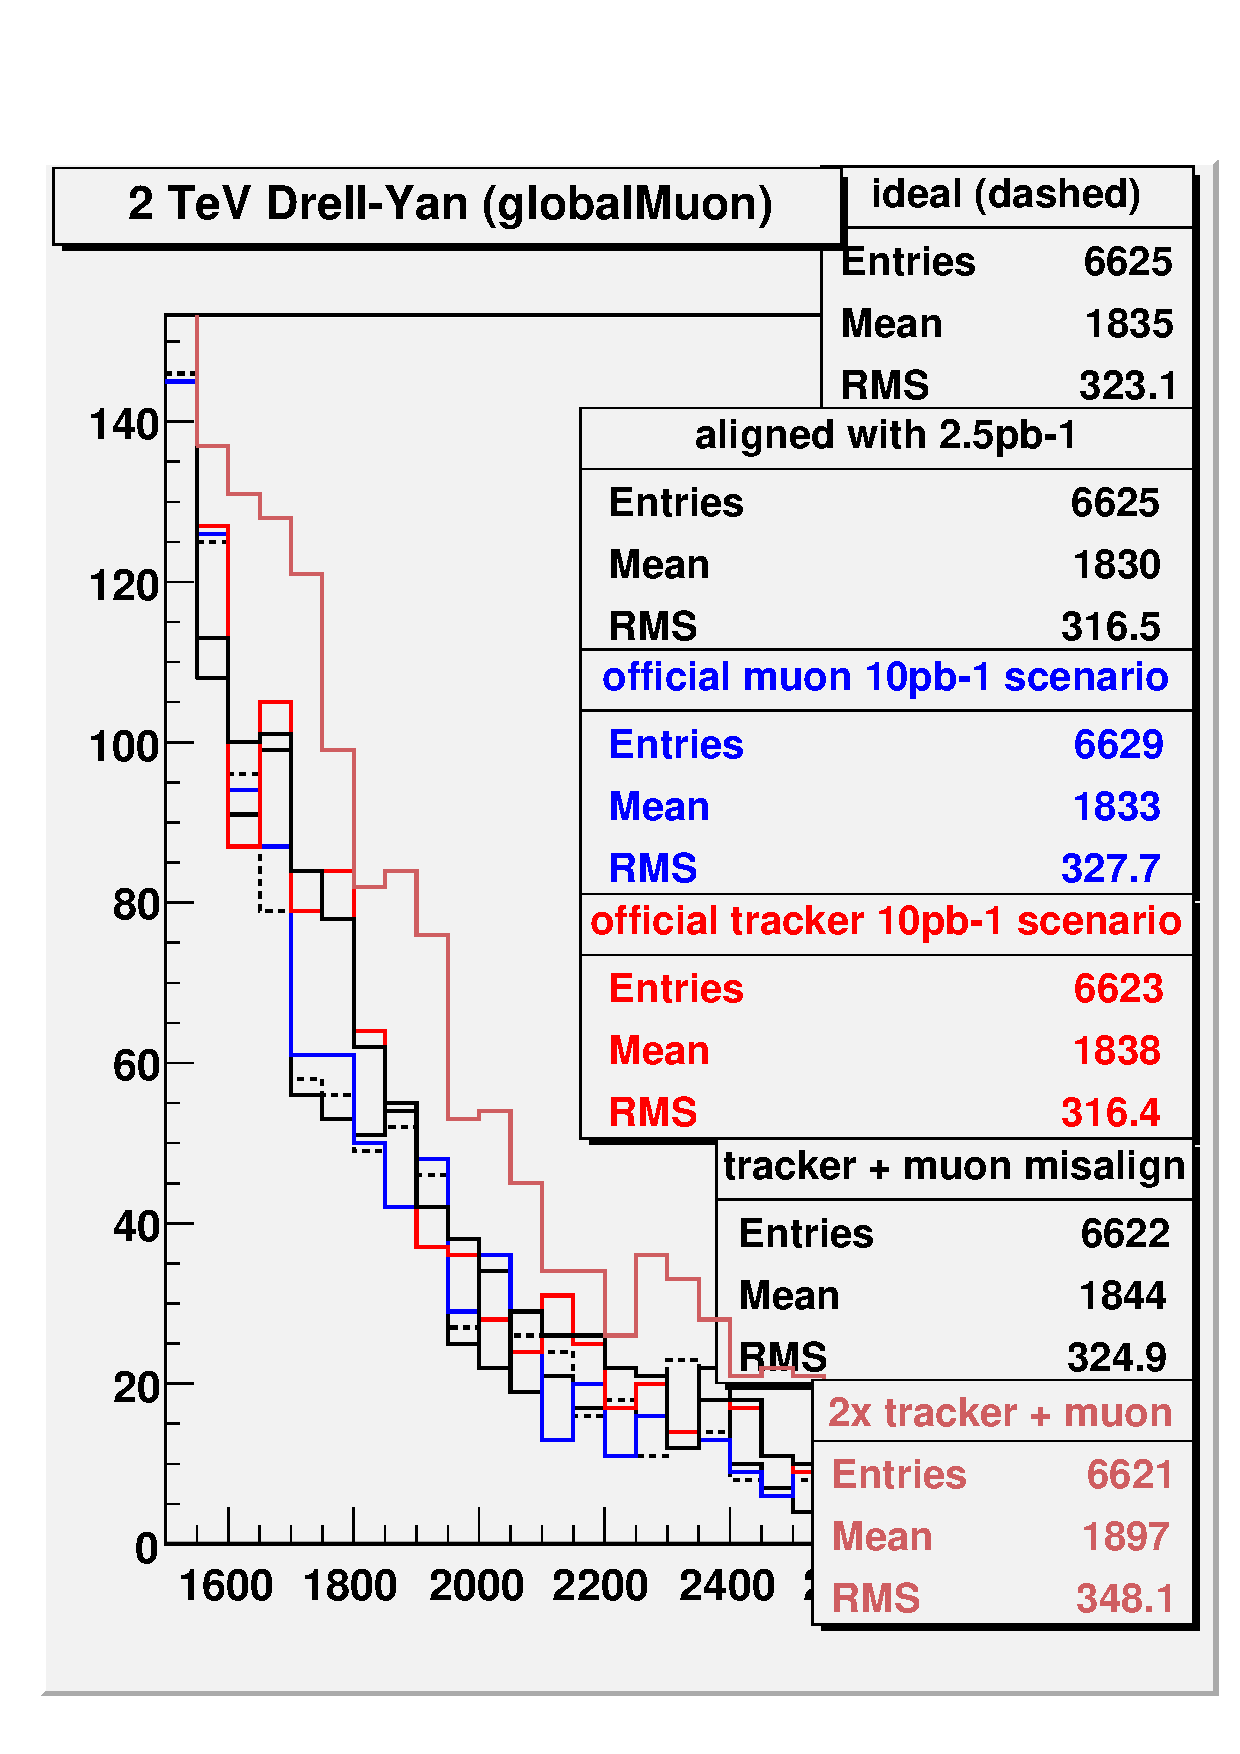
\includegraphics[width=0.85\linewidth]{trackercompare_dy_1000.pdf}}
\column{0.5\linewidth}
\only<1>{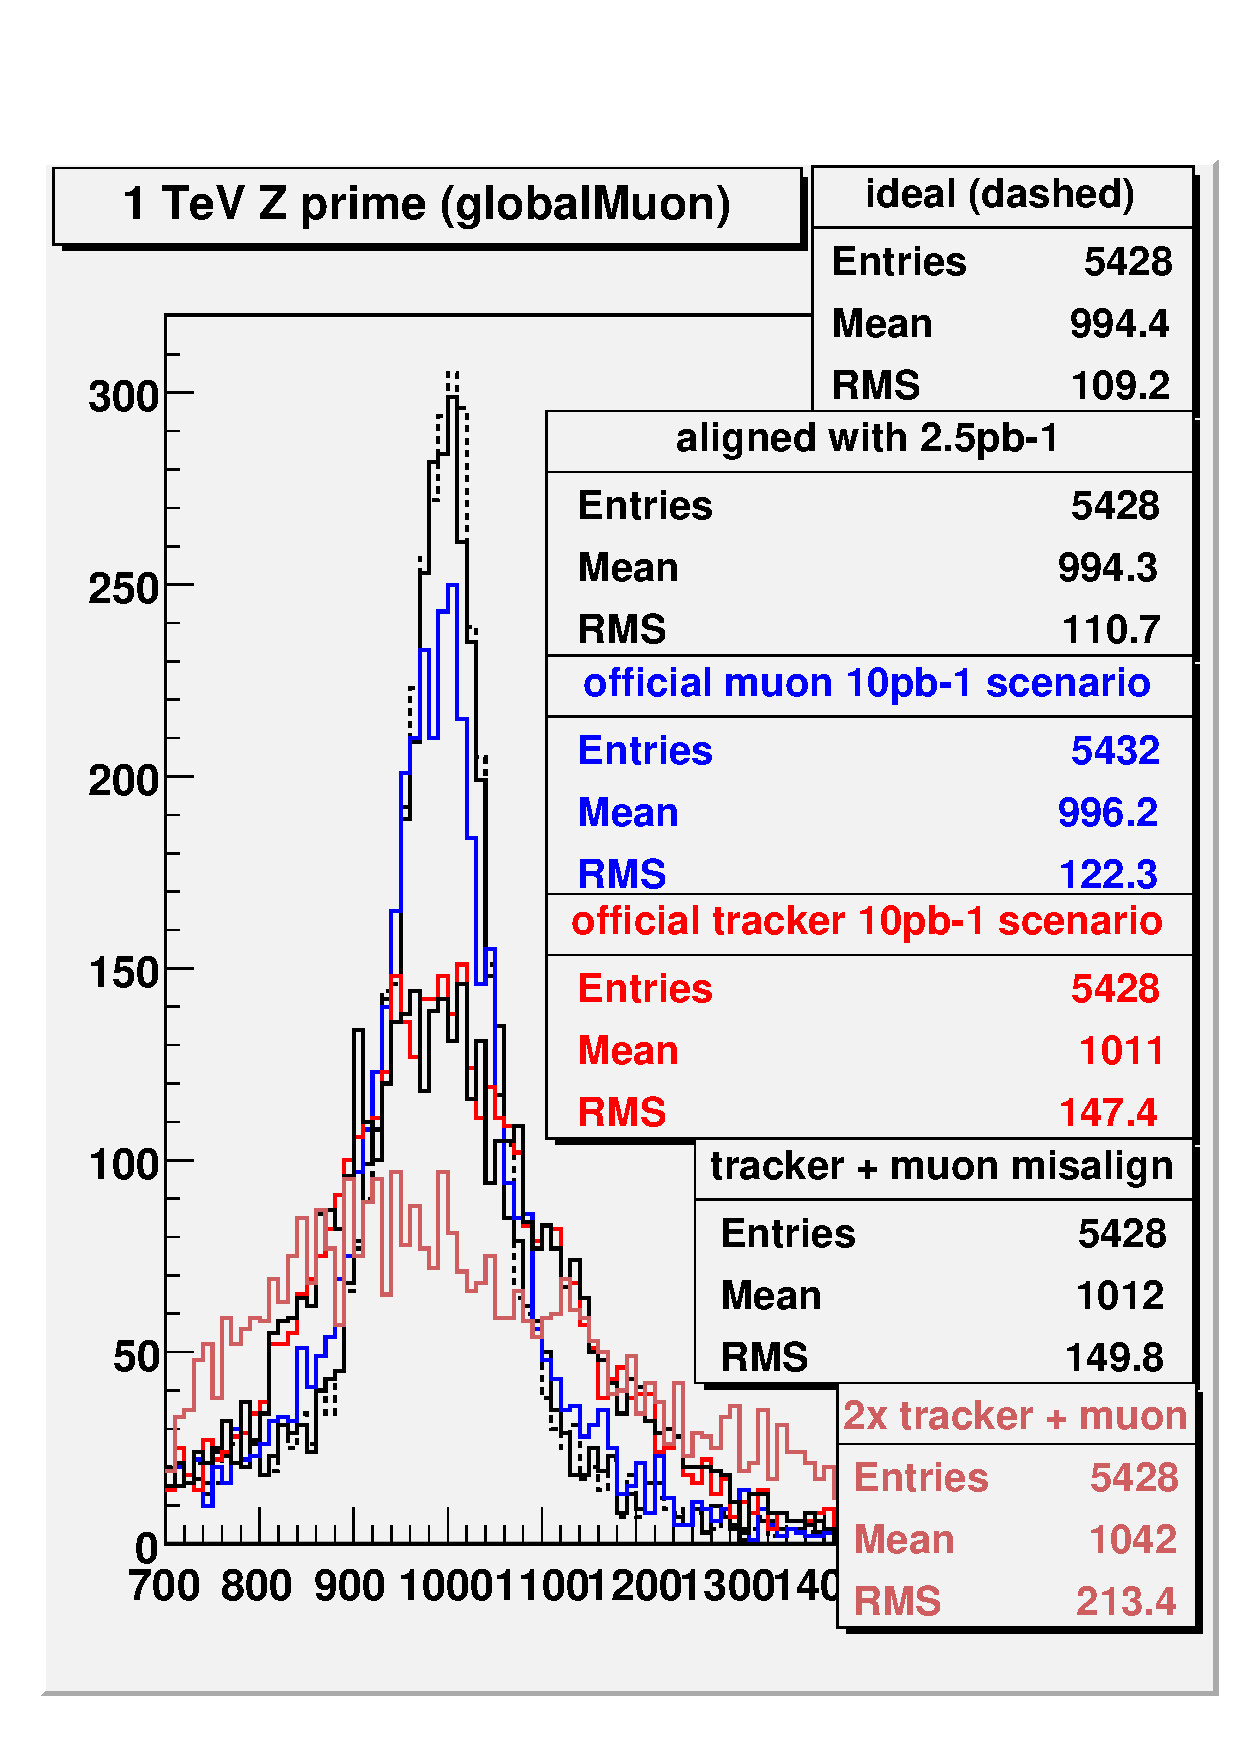
\includegraphics[width=0.85\linewidth]{trackercompare_zprime_1000.pdf}}
\only<2>{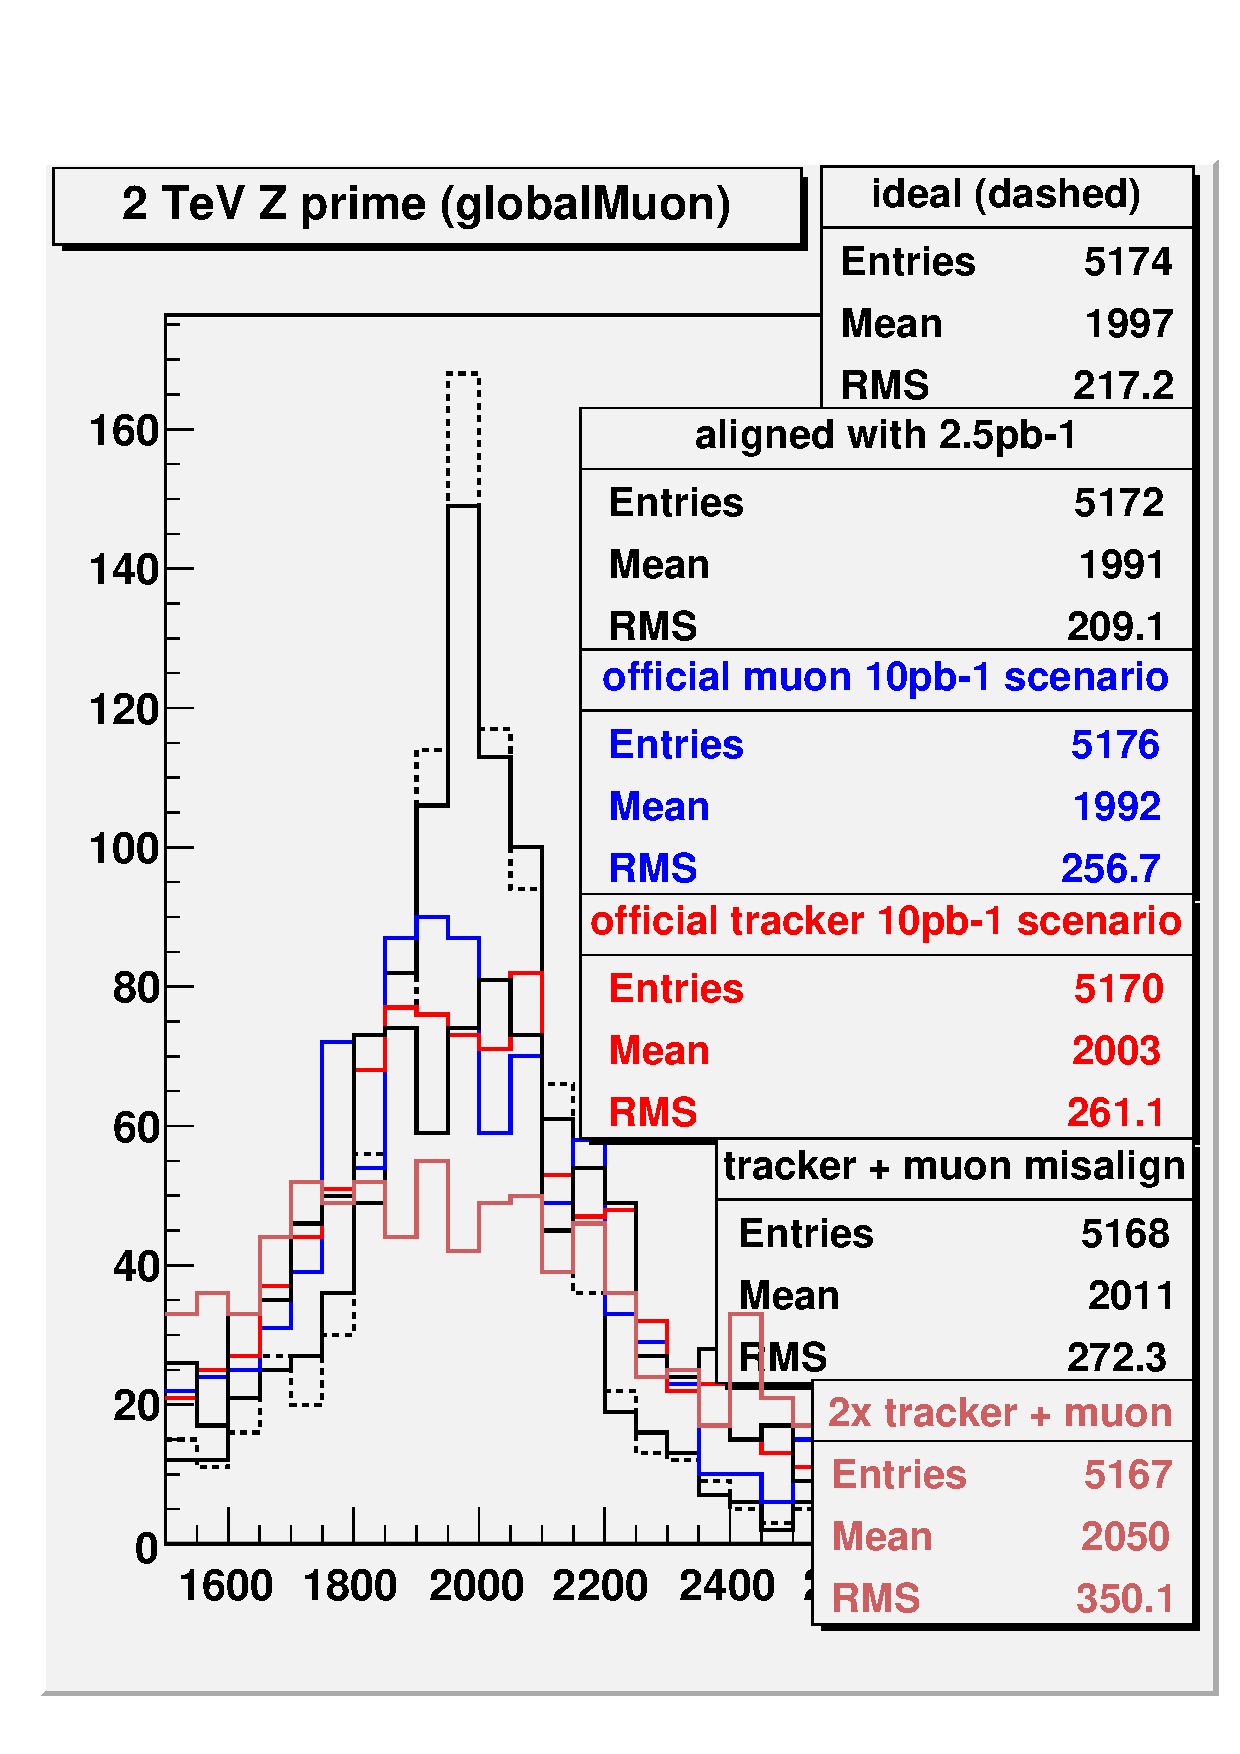
\includegraphics[width=0.85\linewidth]{trackercompare_zprime_2000.pdf}}
\end{columns}

\vspace{0.25 cm}
How realistic is the tracker 10~pb$^{-1}$ scenario?

CSA07 (scaled by $\sqrt{N}$) is 0.1--15$\times$ better, depending on parameter
\end{frame}

%% \begin{frame}
%% \frametitle{Using effect on TeV muons as ``alignment quality''}
%% \begin{center}
%% RMS of event-by-event $\displaystyle \frac{\mbox{misaligned di-muon mass}}{\mbox{ideal di-muon mass}} - 1$
%% \end{center}

%% \renewcommand{\arraystretch}{1.2}
%% \begin{tabular}{c c c c c}
%% Source of alignment & $Z'$(1000) & $Z'$(2000) & \hspace{-0.1cm}DY($>$500)\hspace{-0.1cm} & \hspace{-0.1cm}DY($>$1000)\hspace{-0.1cm} \\\hline
%% 1k $\mu$ (0.25~pb$^{-1}$) & 6.0\% & 5.5\% & 4.8\% & 6.6\% \\
%% 10k $\mu$ (2.5~pb$^{-1}$) & 1.8\% & 1.7\% & 1.6\% & 2.1\% \\
%% 100k $\mu$ (25~pb$^{-1}$) & 1.2\% & 1.1\% & 1.0\% & 1.3\% \\
%% 325k $\mu$ (82~pb$^{-1}$) & 1.0\% & 1.0\% & 0.7\% & 1.2\% \\\hline
%% $|\vec{p}|$ $>$ 60~GeV & 1.0\% & 1.0\% & 0.8\% & 1.2\% \\
%% 20 $<$ $|\vec{p}|$ $<$ 60~GeV & 1.7\% & 1.7\% & 1.5\% & 2.1\%
%% \end{tabular}

%% \vfill\vfill With this as a bottom line, we can make statements like
%% ``switching to $|\vec{p}|$ $>$ 60~GeV is as good as getting a factor of
%% ten more tracks.''
%% \end{frame}

\begin{frame}
\frametitle{Effect of \only<1>{muon}\only<2>{tracker} misalignment on single-track momenta}
\begin{columns}
\column{0.8\linewidth}
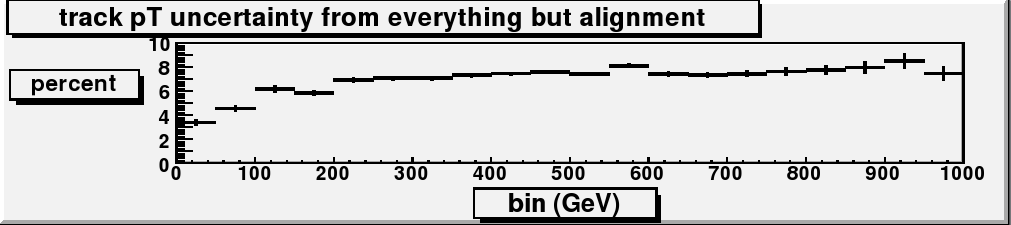
\includegraphics[width=\linewidth]{track_uncertainty_from_all_but_alignment.png}

\only<1>{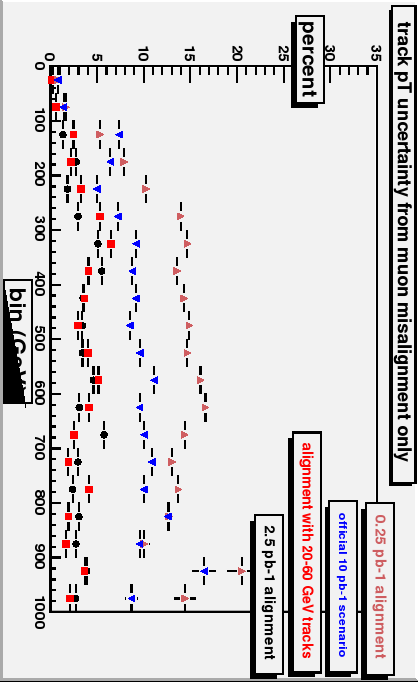
\includegraphics[height=\linewidth, angle=90]{track_uncertainty_from_muon_misalignment.png}}
\only<2>{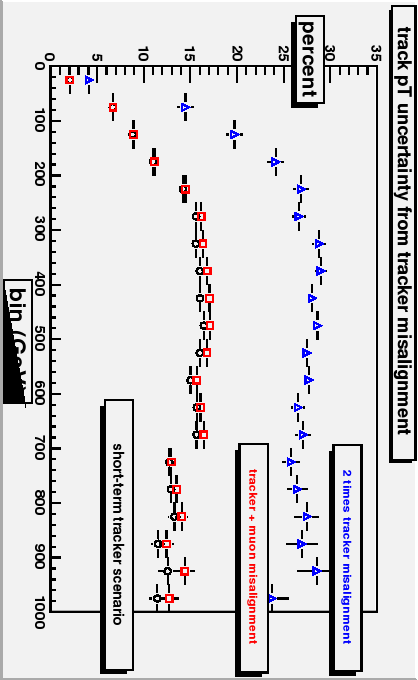
\includegraphics[height=\linewidth, angle=90]{track_uncertainty_from_tracker_misalignment.png}}

\column{0.3\linewidth}
everything but alignment

\vspace{1.5 cm}
effect of alignment only

\vspace{1.5 cm}
$\displaystyle \bigg(\frac{\sigma_{p_T}}{p_T}\bigg) = \bigg(\frac{\sigma_\kappa}{\kappa}\bigg)$

\vspace{0.1 cm}
\mbox{$=$ sum in quadrature} \mbox{of both uncertainties}
\end{columns}
\end{frame}

\section*{}

\begin{frame}
\hspace{-0.83 cm} \textcolor{darkblue}{\Large Conclusions}
\begin{itemize}
\item Stable baseline muon alignment procedure, ready to apply to physics
\item Realistic simulations yield significantly higher-quality alignments than the standard scenario
\item Drell-Yan backgrounds are not strongly affected
\end{itemize}

\vfill
\hspace{-0.83 cm} \textcolor{darkblue}{\Large Ongoing work}
\begin{itemize}
\item Use tracker CSA07 output as a starting point for muon alignment
\item Apply to Dmitry Bourilkov's \textcolor{blue}{\href{https://hypernews.cern.ch/HyperNews/CMS/get/susybsm-hepairs/53.html}{1\_6 $Z'$/Drell-Yan samples}}
\item Fully reconstruct with new geometry, rather than refitting existing tracks
\item Contribute to TeV muon analysis note by validating toy MC alignment
\end{itemize}

\label{numpages}
\end{frame}

\section*{Backup slides}

\begin{frame}
\begin{center}
\Huge \textcolor{blue}{Backup slides}
\end{center}
\end{frame}

\begin{frame}
\frametitle{Dependence on muon momentum}

\vspace{-1 cm}
\mbox{ } \hfill 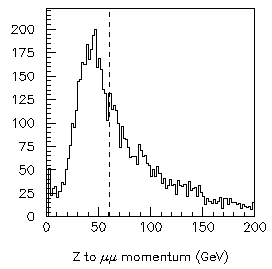
\includegraphics[width=2 cm]{p_distribution.png}

\vspace{-1.3 cm}
\begin{columns}
\column{0.5\linewidth}
\begin{minipage}{2\linewidth}
Radial (local $y$) residual misalignments
\end{minipage}

\vspace{0.1 cm}
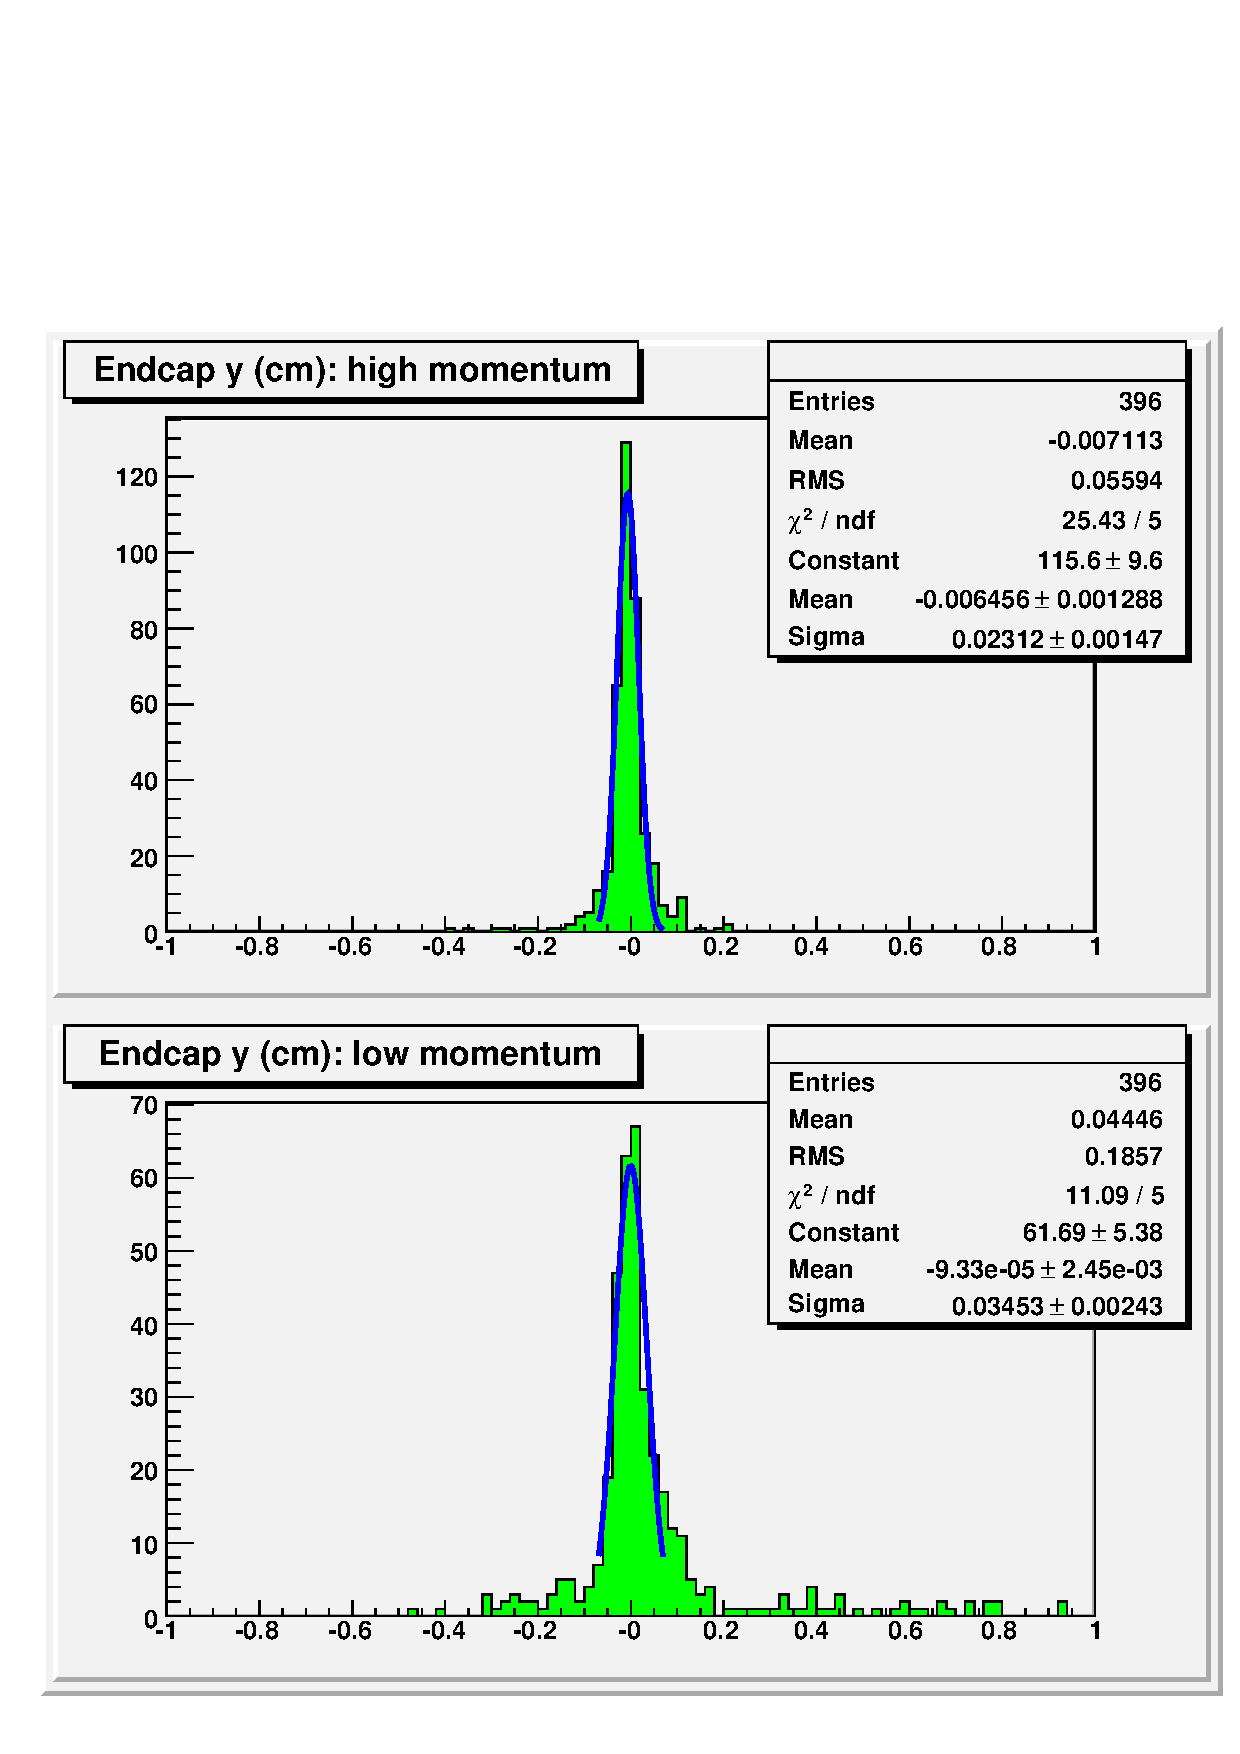
\includegraphics[width=\linewidth]{momentum_endcap_y.pdf}

\column{0.5\linewidth}

\vspace{1 cm}
\begin{itemize}
\item Divide $Z\to\mu\mu$ sample along 60~GeV median
\item Effect on barrel: $<$ 5\% in each parameter
\item Effect on endcap: low-momentum sample has 1.5--3~times worse alignment
\end{itemize}

\vspace{0.2 cm}
Note asymmetric tail!

\vspace{-0.4 cm}
\begin{center}
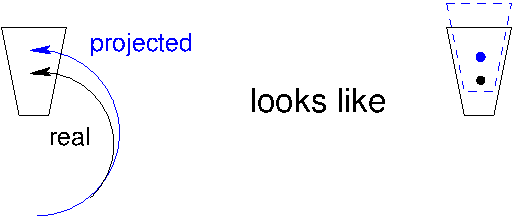
\includegraphics[width=0.8\linewidth]{momentum_y_explanation.pdf}
\end{center}
\end{columns}
\end{frame}

\end{document}
